% =====================================================================
%  Sustentación — Proyecto final de Matemáticas Discretas (MAT 4021)
%  Predicción de brotes de dengue en el Atlántico con un grafo de
%  municipios y una red neuronal.
%
%  Repositorio: https://github.com/Scastanedad/Proyecto-Final-Discretas
%  Compilar:  pdflatex diapositivas  (dos veces). Figuras en figuras/.
%  \quientrue muestra en el pie quién expone cada diapositiva (para ensayar).
%  Notas del orador: cambiar "hide notes" por "show notes on second screen".
% =====================================================================
\documentclass[aspectratio=169,10pt]{beamer}

\usepackage[T1]{fontenc}
\usepackage[utf8]{inputenc}
\IfFileExists{lmodern.sty}{\usepackage{lmodern}}{}
\IfFileExists{spanish.ldf}{\usepackage[spanish,es-nodecimaldot]{babel}}{}
\usepackage{amsmath,amssymb}
\usepackage{booktabs}
\usepackage{tikz}
\usetikzlibrary{arrows.meta,positioning,calc,patterns}

\setbeameroption{hide notes}

% ---------------- Integrantes ----------------
\newcommand{\pA}{Samuel Castañeda}
\newcommand{\pB}{Amir Diago}
\newcommand{\pC}{Andrés Mendible}

% ---------------- Colores (los de las figuras del informe) ----------------
\definecolor{azul}{HTML}{1F5C8B}
\definecolor{azulclaro}{HTML}{9DC3E0}
\definecolor{naranja}{HTML}{D98229}
\definecolor{gris}{HTML}{6B6B6B}
\definecolor{fondoclaro}{HTML}{EEF4F9}

\usecolortheme{default}
\setbeamercolor{structure}{fg=azul}
\setbeamercolor{frametitle}{fg=azul}
\setbeamercolor{block title}{bg=azul,fg=white}
\setbeamercolor{block body}{bg=fondoclaro,fg=black}
\setbeamercolor{alerted text}{fg=naranja}
\setbeamercolor{item}{fg=naranja}
\setbeamertemplate{navigation symbols}{}
\setbeamertemplate{itemize items}[circle]
\setbeamertemplate{blocks}[rounded][shadow=false]
\setbeamerfont{frametitle}{size=\Large,series=\bfseries}
\setbeamerfont{block title}{size=\small,series=\bfseries}
\setbeamersize{text margin left=0.9cm,text margin right=0.9cm}
\setlength{\leftmargini}{1.1em}

\setbeamertemplate{frametitle}{%
  \vspace{0.35cm}\hspace*{-0.1cm}%
  {\usebeamerfont{frametitle}\usebeamercolor[fg]{frametitle}\insertframetitle\par}%
  \vspace{-0.15cm}\hspace*{-0.1cm}\textcolor{naranja}{\rule{1.8cm}{2pt}}\par\vspace{0.1cm}}

% ---------------- Pie de página con quién habla ----------------
\newif\ifquien \quienfalse
\newcommand{\orador}{}
\newcommand{\persona}[2]{\renewcommand{\orador}{Persona #1 · #2}}
\setbeamertemplate{footline}{%
  \leavevmode\hbox{\begin{beamercolorbox}[wd=\paperwidth,ht=2.6ex,dp=1.2ex,leftskip=0.9cm,rightskip=0.9cm]{footline}%
    \scriptsize\color{gris}MAT 4021 · Dengue en el Atlántico\hfill
    \ifquien\orador\quad\fi\insertframenumber
  \end{beamercolorbox}}}

% ---------------- Estilos TikZ ----------------
\tikzset{
  mun/.style={circle,draw=azul,fill=azulclaro,minimum size=0.85cm,inner sep=0pt,font=\scriptsize\bfseries},
  neurona/.style={circle,draw=azul,fill=azulclaro,minimum size=0.28cm,inner sep=0pt},
  salida/.style={circle,draw=naranja,fill=naranja!60,minimum size=0.34cm,inner sep=0pt},
}
\newcommand{\cifra}[2]{{\LARGE\bfseries\color{naranja}#1}\\[-3pt]{\footnotesize #2}}

\title{¿Dónde fumigar primero?}
\subtitle{Predicción de brotes de dengue en los municipios del Atlántico\\con un grafo de municipios vecinos y una red neuronal}
\author{\pA\\\pB\\\pC}
\institute{MAT 4021 Matemáticas Discretas · Grupo 4 · Prof. Iván Gómez\\Universidad del Norte}
\date{15 de noviembre de 2026}

\begin{document}

% =====================================================================
%  PERSONA 1  (≈ 2:40)  — diapositivas 1, 2, 3 y 8 (cierre)
% =====================================================================

% ---- 1. Portada (0:15) ----
\persona{1}{\pA}
\begin{frame}[plain]
  \vspace{0.5cm}
  \begin{minipage}[t]{0.62\textwidth}
    {\color{naranja}\rule{1.8cm}{2pt}}\\[6pt]
    {\raggedright\Huge\bfseries\color{azul}¿Dónde fumigar primero?\\[8pt]}
    {\large Predicción de brotes de dengue en los municipios del Atlántico con un grafo de municipios vecinos y una red neuronal}\\[14pt]
    {\small\pA\\\pB\\\pC}\\[8pt]
    {\footnotesize\color{gris} MAT 4021 Matemáticas Discretas · Grupo 4 · Prof.\ Iván Gómez\\Universidad del Norte}\\[8pt]
    {\scriptsize\href{https://github.com/Scastanedad/Proyecto-Final-Discretas}{\color{azul}\texttt{github.com/Scastanedad/Proyecto-Final-Discretas}}}
  \end{minipage}\hfill
  \begin{minipage}[t]{0.33\textwidth}
    \vspace{-1.2cm}\hfill
    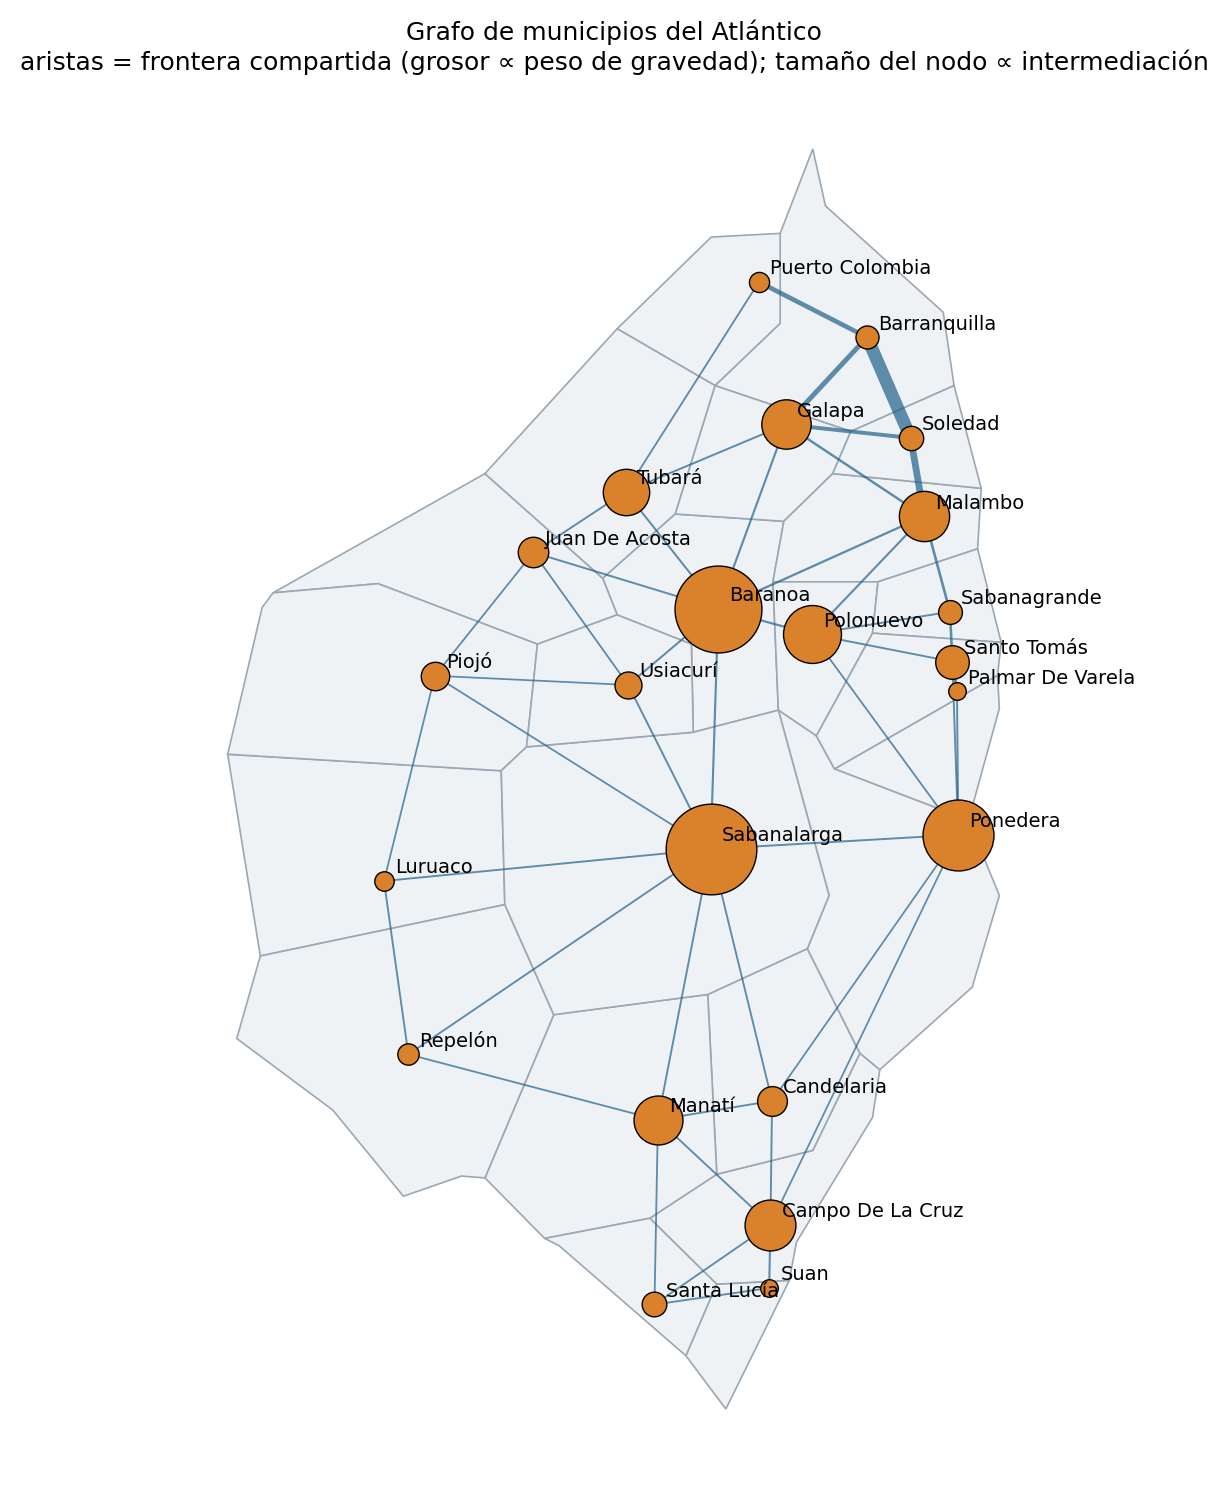
\includegraphics[height=7.2cm]{figuras/grafo_atlantico.png}
  \end{minipage}
  \note{0:15. Si los recursos para fumigar son limitados, ¿en qué municipio del Atlántico conviene intervenir primero?}
\end{frame}

% ---- 2. Problema + datos (1:05) ----
\persona{1}{\pA}
\begin{frame}{El problema: recursos limitados, contagio sin fronteras}
  \begin{columns}[T]
    \begin{column}{0.36\textwidth}
      \cifra{49.308}{casos de dengue, 2018--2025}\\[2pt]
      \cifra{2,87 M}{habitantes en 23 municipios}\\[2pt]
      \cifra{12}{municipios en brote (sem. 19 de 2026)}
    \end{column}
    \begin{column}{0.64\textwidth}
      \centering
      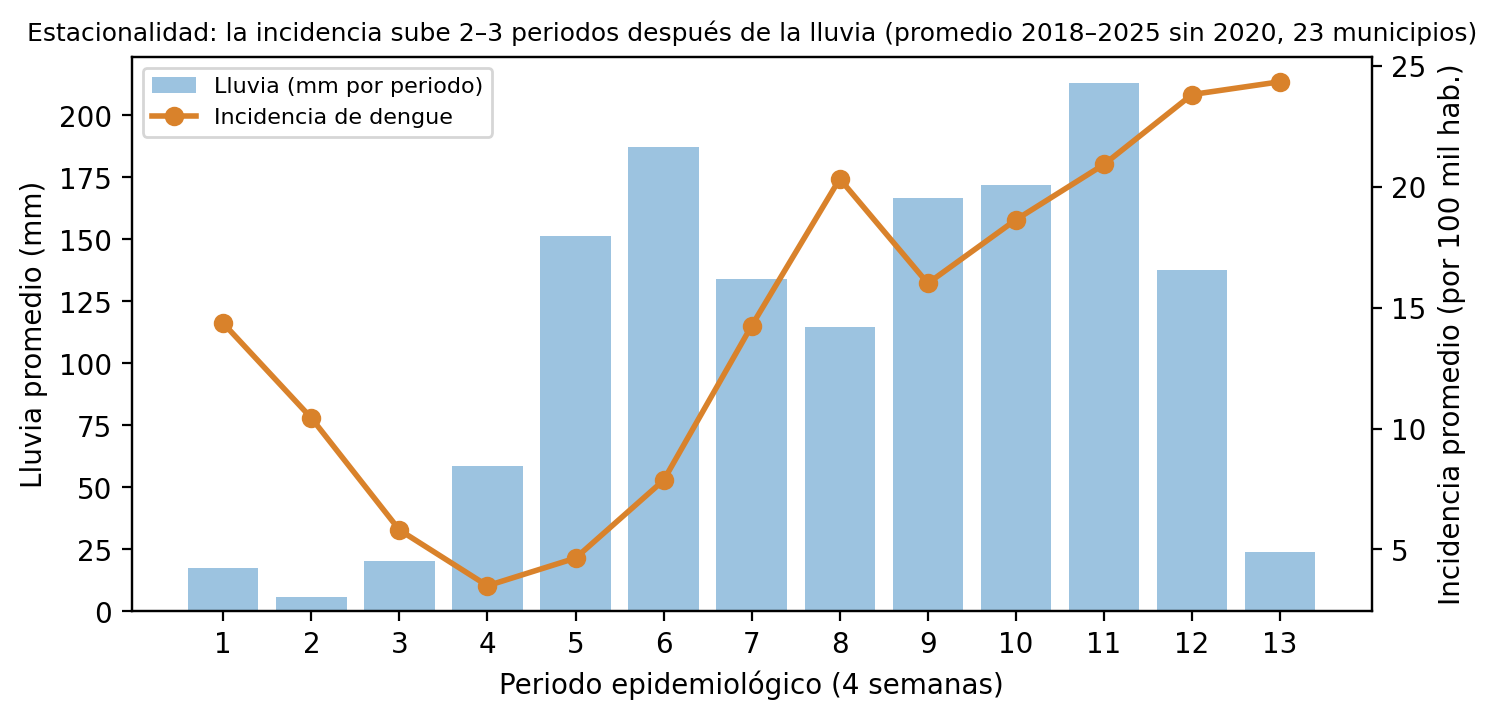
\includegraphics[height=3.4cm]{figuras/estacionalidad.png}\\[2pt]
      {\scriptsize Datos públicos: \textbf{SIVIGILA} (casos), \textbf{DANE} (población, límites), \textbf{Open-Meteo} (clima). Periodos de 4 semanas: 2.392 filas.\\
      Correlación lluvia--incidencia: $\rho=0{,}06$ sin rezago, \alert{$\rho=0{,}30$ con 2 periodos de rezago}.}
    \end{column}
  \end{columns}
  \vspace{0.15cm}
  \begin{block}{Nuestra pregunta}
    Anticipar los brotes \alert{un periodo (4 semanas) antes} y decidir \alert{en qué orden intervenir}, usando que las personas, y el virus, se mueven entre municipios vecinos.
  \end{block}
  \note{1:05. Hoy se reacciona cuando el brote ya está. El contagio no respeta límites municipales: por eso un grafo. Cumple las 4 condiciones de impacto: afecta a alguien, hay evidencia, se puede mejorar, se puede modelar. Datos 100 \% reales y públicos. Con semanas sueltas el 57 \% de las celdas eran cero; con 4 semanas baja a 35 \%. El dengue sube 2-3 periodos tras la lluvia (ciclo del mosquito): por eso la red recibe lluvia rezagada hasta t-3.}
\end{frame}

% ---- 3. Brote y validación (0:45) ----
\persona{1}{\pA}
\begin{frame}{¿Qué es un brote? ¿Cómo evitamos hacer trampa?}
  \begin{block}{Definición de brote en el municipio $m$, periodo $t$}
    \[\mathrm{inc}_m(t) > \mu_{m,p(t)} + s_{m,p(t)}\quad\text{y}\quad \text{casos}_m(t)\geq 3\]
    \footnotesize $\mu,s$: media y desviación de la incidencia en los años de entrenamiento, para ese mismo periodo del año.
  \end{block}
  \vspace{0.15cm}
  \centering
  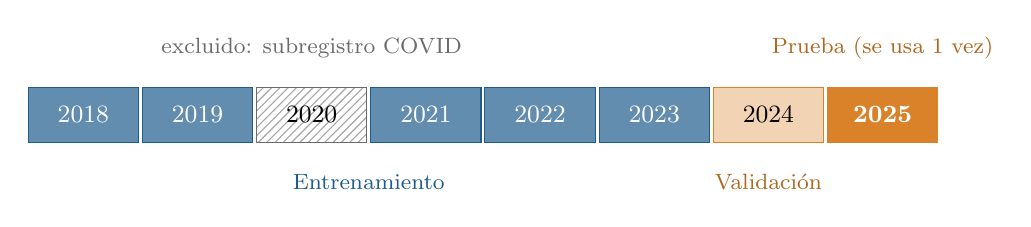
\begin{tikzpicture}[x=1.45cm,y=1cm]
    \foreach \a/\k in {0/2018,1/2019,3/2021,4/2022,5/2023}{
      \node[draw=azul,fill=azul!70,text=white,minimum width=1.4cm,minimum height=0.7cm,font=\small] at (\a,0) {\k};}
    \node[draw=gris,pattern=north east lines,pattern color=gris!60,minimum width=1.4cm,minimum height=0.7cm,font=\small] at (2,0) {2020};
    \node[draw=naranja,fill=naranja!35,minimum width=1.4cm,minimum height=0.7cm,font=\small] at (6,0) {2024};
    \node[draw=naranja,fill=naranja,text=white,minimum width=1.4cm,minimum height=0.7cm,font=\small\bfseries] at (7,0) {2025};
    \node[font=\footnotesize,text=azul] at (2.5,-0.85) {Entrenamiento};
    \node[font=\footnotesize,text=gris] at (2,0.85) {excluido: subregistro COVID};
    \node[font=\footnotesize,text=naranja!80!black] at (6,-0.85) {Validación};
    \node[font=\footnotesize,text=naranja!80!black] at (7,0.85) {Prueba (se usa 1 vez)};
  \end{tikzpicture}
  \vspace{0.1cm}
  \begin{itemize}\setlength\itemsep{2pt}
    \item División \alert{por años, nunca al azar}: el modelo no ve el futuro.
    \item Umbral de alerta elegido en 2024 con $F_2$: no detectar un brote es peor que una falsa alarma.
    \item Red entrenada con \alert{20 semillas}: reportamos media $\pm$ desviación.
  \end{itemize}
  \note{0:45. 2020 se excluye: los casos se desplomaron desde marzo (Barranquilla de 461 a 9-27 por periodo). 2021 se conserva: tuvo un brote real a fin de año. Sobremuestreo en entrenamiento por desbalance (15,5 \% de brotes).}
\end{frame}

% =====================================================================
%  PERSONA 2  (≈ 2:50)  — diapositivas 4 y 5
% =====================================================================

% ---- 4. Grafo + puentes (1:25) ----
\persona{2}{\pB}
\begin{frame}{El grafo: los puentes no son los que más casos tienen}
  \begin{columns}[c]
    \begin{column}{0.56\textwidth}
      \begin{block}{$G=(V,E,w)$}
        \footnotesize
        \begin{itemize}\setlength\itemsep{1pt}
          \item $V$: los \textbf{23 municipios}
          \item $\{a,b\}\in E$ si comparten $\geq 1$ km de frontera (polígonos del DANE): \textbf{47 aristas}, grafo conexo
          \item Peso de gravedad: $w(a,b)\propto \dfrac{P_a\,P_b}{d(a,b)^2}$
        \end{itemize}
      \end{block}
      \vspace{-2pt}
      \centering\scriptsize
      \begin{tabular}{lrrr}
        \toprule
        Municipio & Grado & Interm. (norm.) & Casos\\
        \midrule
        \textbf{Sabanalarga} & 8 & \textbf{0,370} & 1.629\\
        \textbf{Baranoa} & 7 & \textbf{0,339} & 1.438\\
        \midrule
        Soledad & 3 & 0,013 & 9.824\\
        Barranquilla & 3 & 0,010 & 27.616\\
        \bottomrule
      \end{tabular}\\[2pt]
      \begin{block}{Lectura}
        \scriptsize Barranquilla concentra el \alert{56 \%} de los casos, pero está en el borde norte. Un contagio hacia el sur debe pasar, en términos de vecindad, por \alert{Sabanalarga y Baranoa}.
      \end{block}
    \end{column}
    \begin{column}{0.44\textwidth}
      \centering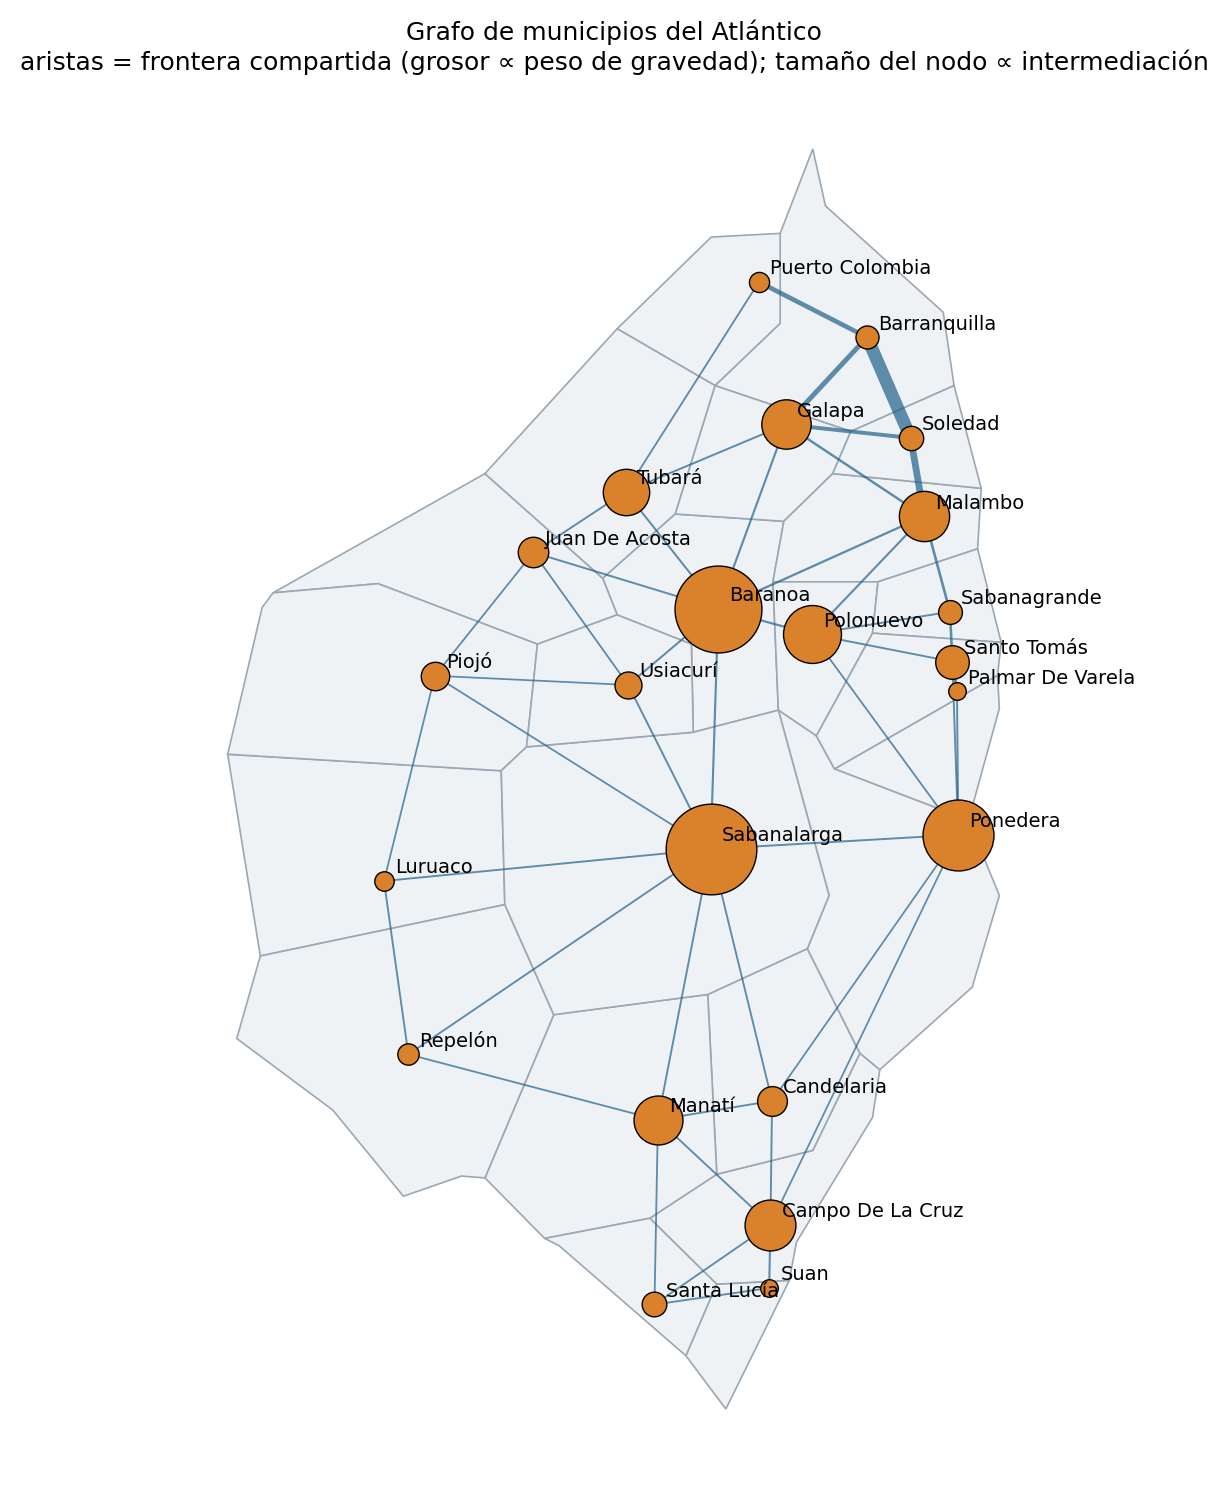
\includegraphics[height=5.3cm]{figuras/grafo_atlantico.png}
    \end{column}
  \end{columns}
  \note{1:25. Las aristas se calculan desde polígonos oficiales, no a ojo (se descartaron 4 contactos de menos de 300 m; el siguiente mide 2,1 km). Mayor peso: Barranquilla--Soledad. Tamaño del nodo = intermediación. Grado dice cuántos vecinos tiene; intermediación dice cuántas rutas de contagio pasan por ahí. Para cortar el contagio importa la segunda. Tabla completa (con cercanía) en el informe, Tabla 5.}
\end{frame}

% ---- 5. Algoritmos + demo (1:25) ----
\persona{2}{\pB}
\begin{frame}[fragile]{Algoritmos propios y verificados a mano}
  \begin{columns}[T]
    \begin{column}{0.50\textwidth}
      \centering
      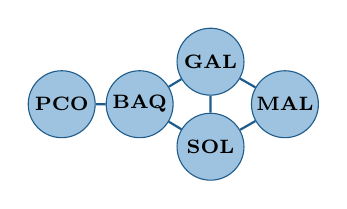
\begin{tikzpicture}[scale=0.45]
        \node[mun] (P) at (0,0) {PCO};
        \node[mun] (B) at (2.2,0) {BAQ};
        \node[mun] (G) at (4.2,1.2) {GAL};
        \node[mun] (S) at (4.2,-1.2) {SOL};
        \node[mun] (M) at (6.3,0) {MAL};
        \draw[azul,thick] (P)--(B) (B)--(G) (B)--(S) (G)--(S) (G)--(M) (S)--(M);
      \end{tikzpicture}\\[4pt]
      \footnotesize
      \begin{tabular}{lccccc}
        \toprule
         & BAQ & SOL & GAL & MAL & PCO\\
        \midrule
        Grado & 3 & 3 & 3 & 2 & 1\\
        Cercanía & 0,800 & 0,800 & 0,800 & 0,571 & 0,500\\
        Intermediación & \textbf{3} & 1 & 1 & 0 & 0\\
        \bottomrule
      \end{tabular}
    \end{column}
    \begin{column}{0.50\textwidth}
      \begin{block}{Intermediación (Freeman)}
        \[B(v)=\sum_{s\neq v\neq t}\frac{\sigma_{st}(v)}{\sigma_{st}}\]
      \end{block}
      \begin{itemize}\setlength\itemsep{2pt}\small
        \item \textbf{BFS} desde cada vértice: distancias y $\sigma_{sv}$
        \item \textbf{Algoritmo de Brandes}, $O(n\,|E|)$
        \item Sin librerías de grafos (\texttt{grafo\_lib.py})
      \end{itemize}
      \alert{\small\textbf{Coincide} con el cálculo a mano y con NetworkX en el grafo completo.}
    \end{column}
  \end{columns}
  \vspace{-6pt}
  \begin{block}{Demostración: terminal}
\footnotesize
\begin{verbatim}
$ python tests/test_grafo.py
OK  test_grado   OK  test_cercania   OK  test_intermediacion
OK  test_presion_vecinos   OK  test_contra_networkx_grafo_completo
\end{verbatim}
  \end{block}
  \note{1:25. Ejemplo BAQ=3: los pares PCO--SOL y PCO--GAL tienen un solo camino más corto, por BAQ (+1 cada uno); PCO--MAL tiene dos caminos (por SOL y por GAL) y ambos pasan por BAQ (+1). Total 3. Brandes: por cada origen un BFS cuenta caminos y luego se acumulan dependencias en orden inverso de distancia. Demo: 11 pruebas automáticas en total (calendario epidemiológico, grafo y sin fuga de información); \texttt{python src/06\_prioridad.py} genera el ranking en ~30 s. Plan B: captura de pantalla por si falla en vivo.}
\end{frame}

% =====================================================================
%  PERSONA 3  (≈ 3:15)  — diapositivas 6 y 7
% =====================================================================

% ---- 6. Red neuronal + resultados (1:30) ----
\persona{3}{\pC}
\begin{frame}{La red neuronal: ¿habrá brote en el próximo periodo?}
  \begin{columns}[T]
    \begin{column}{0.46\textwidth}
      \textbf{14 entradas} por municipio:
      \begin{itemize}\setlength\itemsep{1pt}\footnotesize
        \item incidencia en $t,\,t{-}1,\,t{-}2$
        \item anomalía de lluvia de $t$ a $t{-}3$
        \item temperatura, humedad y periodo del año
        \item población (logaritmo)
        \item \alert{presión de vecinos} (del grafo): promedio de la incidencia de los vecinos ponderado por $w$
      \end{itemize}
      \vspace{3pt}
      \centering
      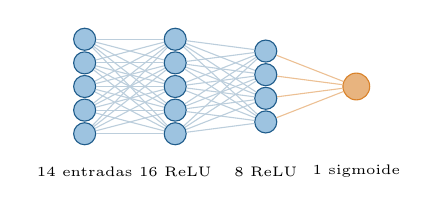
\begin{tikzpicture}[x=1.15cm,y=0.3cm]
        \foreach \l/\n/\x in {0/5/0,1/5/1,2/4/2}{
          \foreach \i in {1,...,\n}{\node[neurona] (n\l\i) at (\x,{(\n+1)/2-\i}) {};}}
        \node[salida] (n31) at (3,0) {};
        \foreach \i in {1,...,5}{\foreach \j in {1,...,5}{\draw[azul!30,thin] (n0\i)--(n1\j);}}
        \foreach \i in {1,...,5}{\foreach \j in {1,...,4}{\draw[azul!30,thin] (n1\i)--(n2\j);}}
        \foreach \i in {1,...,4}{\draw[naranja!50,thin] (n2\i)--(n31);}
        \node[font=\tiny,align=center] at (0,-3.6) {14 entradas};
        \node[font=\tiny,align=center] at (1,-3.6) {16 ReLU};
        \node[font=\tiny,align=center] at (2,-3.6) {8 ReLU};
        \node[font=\tiny,align=center] at (3,-3.6) {1 sigmoide};
      \end{tikzpicture}
    \end{column}
    \begin{column}{0.54\textwidth}
      \footnotesize
      \centering
      \begin{tabular}{lccc}
        \toprule
        Prueba 2025 & Detecta brotes & Precisión & AUC-ROC\\
        \midrule
        Persistencia & 68 \% & \textbf{0,72} & 0,77\\
        Reg.\ logística & 85 \% & 0,52 & \textbf{0,84}\\
        \textbf{Red neuronal} & \textbf{88 \%} & 0,52 & \textbf{0,84}\\
        \bottomrule
      \end{tabular}\\[2pt]
      {\tiny Persistencia: ``si hay brote, seguirá habiendo''. Red: media de 20 semillas.}\\[6pt]
      \cifra{88 \%}{de los brotes detectados un periodo antes, frente a 68 \% de la regla simple}
      \begin{itemize}\setlength\itemsep{2pt}\footnotesize\raggedright
        \item \textbf{Costo:} cerca de la mitad de las alertas son falsas: por cada brote real se fumigaría un municipio de más.
        \item \textbf{Pero:} la red \alert{empata} con la regresión logística; con ${\sim}1.400$ filas no hay datos para que una red gane.
      \end{itemize}
    \end{column}
  \end{columns}
  \note{1:30. Arquitectura 14-16-8-1, ReLU, sigmoide, entropía cruzada con L2, Adam. Prueba: 299 filas, 100 brotes. Se repiten ejemplos de brote en entrenamiento (sobremuestreo) para que no aprenda a decir siempre ``no'': con 15 \% de brotes, decir siempre ``no'' daría 85 \% de exactitud y no sirve; por eso F2. El umbral se eligió privilegiando la sensibilidad, por eso la precisión baja de 0,72 a ~0,50.}
\end{frame}

% ---- 7. Grafo: predecir vs decidir (1:45) ----
\persona{3}{\pC}
\begin{frame}{El grafo no ayudó a predecir, pero sí a decidir}
  \begin{columns}[T]
    \begin{column}{0.47\textwidth}
      \begin{block}{Predecir: el grafo no ayudó}
        \small
        \cifra{$-0{,}005\pm0{,}031$}{diferencia en AUC-PR (red con grafo $-$ sin grafo); el grafo gana en \textbf{7 de 20} semillas}\\[4pt]
        \textbf{¿Por qué?}
        \begin{enumerate}\setlength\itemsep{1pt}\footnotesize
          \item La incidencia propia ya resume casi todo (correlación parcial de los vecinos: 0,18).
          \item Los brotes son \alert{casi simultáneos}: mismo clima, misma temporada.
          \item El grafo solo incluye vecinos \emph{dentro} del Atlántico.
        \end{enumerate}
        {\scriptsize Tampoco ayudó en los 17 municipios con pocos casos (AUC-ROC 0,827 con grafo vs.\ 0,833 sin grafo).}
      \end{block}
    \end{column}
    \begin{column}{0.53\textwidth}
      \begin{block}{Decidir: priorizar la fumigación}
        \small
        \[\hat P(\text{brote}_v)\times\Bigl(1+\tfrac{B(v)}{\max_u B(u)}\Bigr)\]
        \centering
        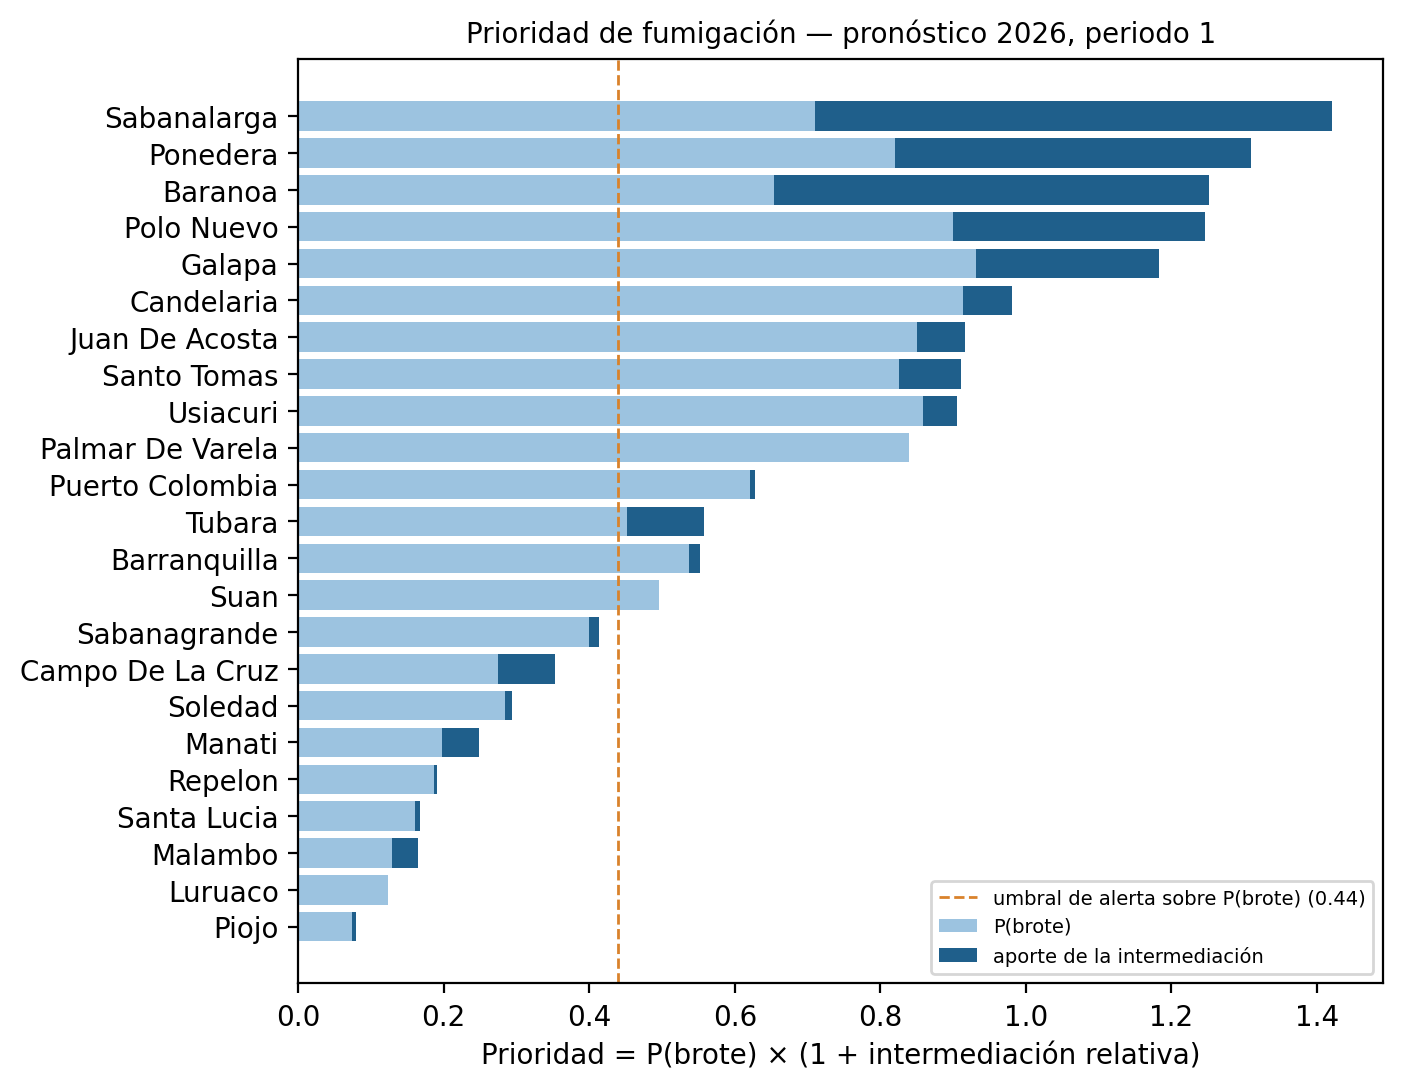
\includegraphics[height=3.8cm]{figuras/prioridad_2026_p1.png}\\[2pt]
        \footnotesize\raggedright\textbf{Top 5, periodo 1 de 2026:} Sabanalarga, Ponedera, Baranoa, Polonuevo, Galapa. La centralidad como mucho duplica la prioridad: el riesgo propio manda.
      \end{block}
    \end{column}
  \end{columns}
  \note{1:45. No ajustamos nada para forzar un resultado: eso sería hacer trampa con los datos de prueba. Medir que no ayuda también es resultado. Predecir no es decidir: si dos municipios tienen riesgo parecido, fumigar primero el que corta más rutas. Sabanalarga y Baranoa suben al 1.º y 3.º puesto aunque su probabilidad no sea la más alta (Galapa 0,93 y Candelaria 0,91 tienen la mayor). 14 de 23 municipios en alerta (umbral 0,44). El pronóstico aún no se puede verificar: el SIVIGILA publica con meses de retraso.}
\end{frame}

% =====================================================================
%  PERSONA 1  — cierre (0:40)
% =====================================================================
\persona{1}{\pA}
\begin{frame}{Conclusiones y limitaciones}
  \begin{itemize}\setlength\itemsep{5pt}
    \item Con datos públicos se anticipa el \alert{88 \%} de los brotes un periodo antes (68 \% con la regla simple).
    \item La lluvia de hace \alert{8 a 12 semanas} es la mejor señal climática.
    \item Una red neuronal pequeña \alert{iguala} a la regresión logística con estos datos.
    \item El grafo \textbf{no mejora la predicción}, pero \textbf{sí mejora la decisión}: los puentes del contagio son Sabanalarga y Baranoa, no Barranquilla.
  \end{itemize}
  \vspace{0.15cm}
  \begin{columns}[T]
    \begin{column}{0.52\textwidth}
      \begin{block}{Limitaciones}
        \footnotesize
        Subregistro por pandemia · casos notificados · clima de modelo numérico · movilidad aproximada con gravedad · sin vecinos de otros departamentos · prioridad no validada con intervenciones reales
      \end{block}
    \end{column}
    \begin{column}{0.48\textwidth}
      \begin{block}{Trabajo futuro}
        \footnotesize
        Datos reales de movilidad para los pesos · incluir municipios vecinos de Magdalena y Bolívar · simulación SIR sobre el grafo
      \end{block}
    \end{column}
  \end{columns}
  \vspace{0.2cm}
  \centering\small Código, datos e instrucciones: \href{https://github.com/Scastanedad/Proyecto-Final-Discretas}{\color{azul}\texttt{github.com/Scastanedad/Proyecto-Final-Discretas}}
  \note{0:40. Cierre. Agradecer y abrir preguntas: cada integrante debe poder responder sobre cualquier diapositiva.}
\end{frame}

\end{document}
